\documentclass[11pt,a4paper]{scrartcl}

\usepackage[english]{babel}
\usepackage{standalone}
\usepackage{layouts}
\usepackage{geometry}
 \geometry{
 a4paper,
 margin=20mm
 }
%\usepackage{showframe}

%--Fonts---%
\newcommand\hmmax{0} %Avoid too many alphabets error
\newcommand\bmmax{0}
\renewcommand{\rmdefault}{ppl} % rm
\linespread{1.05}        % Palatino needs more leading
\usepackage[scaled]{helvet} % ss
\usepackage{courier} % tt
\usepackage{mathpazo} 
\usepackage{microtype}

%---Encoding---%
\usepackage[utf8]{inputenc}
\usepackage[T1]{fontenc}
\usepackage{lmodern}
\usepackage{csquotes}
\usepackage[ddmmyyyy,hhmmss]{datetime} %Compilation date

%---Math---%
\usepackage{amsmath,amsthm,amstext,amsbsy,amsfonts,amssymb,stackengine}
\usepackage{mathrsfs}
\usepackage{cancel}
\usepackage{bm}
\usepackage{mathtools}
\usepackage{mathdots}
\usepackage{thmtools}
\usepackage{array}
\usepackage{yhmath}
\usepackage{gensymb}
\usepackage{blkarray}
\usepackage{xfrac}

%---Plots---%
\usepackage{epstopdf}
\usepackage{gnuplottex}
\usepackage{calc}
\usepackage{graphicx}
\usepackage{color}
\usepackage{transparent}

%---Physics---%
\usepackage{physics}
\usepackage{siunitx}
\sisetup{
separate-uncertainty = true
}

%---Tables---%
\usepackage{booktabs}
\usepackage{multirow}

\setlength{\aboverulesep}{0pt} %removes annoying spaces in booktabs tables
\setlength{\belowrulesep}{0pt}
\setlength{\extrarowheight}{.75ex}
\setlength\parindent{0pt} 

%---Graphics & Plots---%
\usepackage{color}
\usepackage[usenames, dvipsnames, table]{xcolor} %colori
\usepackage{wrapfig}
\usepackage[font=footnotesize, labelfont=bf,
            labelformat=parens,
            labelsep=endash, justification=raggedright,
            singlelinecheck=on]{caption} %fancy captions
\usepackage{subcaption} 
\usepackage{pgf,tikz}
\usetikzlibrary{arrows}
\usetikzlibrary{tikzmark}
\usetikzlibrary{patterns}
\usepackage{soul}
\usepackage[framemethod=tikz]{mdframed}
\usepackage{fancybox}
\usepackage{framed}

%---Indeces, links, bibliography---%
\usepackage{imakeidx} %Indice analitico
\usepackage[stable]{footmisc}

%\usepackage{xr-hyper}
\PassOptionsToPackage{hyphens}{url}\usepackage{hyperref}  %hyperref va caricato sempre dopo footmisc, altrimenti le footnotes si buggano e riportano tutte alla prima pagina
%\usepackage[inline]{showlabels} %Draft

\usepackage[symbol=$\wedge$,numberlinked=false]{footnotebackref}
\makeindex[columns=2, title=Analytical index, options= -s indexstyle.ist]

\usepackage[backend=biber,sorting=none]{biblatex}
\renewbibmacro{in:}{}
\addbibresource{bibliography.bib}

%---Utilities---%
\usepackage{comment}
\usepackage{xspace}
\usepackage{marginnote}
\usepackage{ragged2e}
\usepackage{enumerate}
\usepackage{enumitem}
\usepackage{etoolbox}
\usepackage{xargs}                      % Use more than one optional parameter in a new commands
\usepackage{lipsum}  
\usepackage{float}

\usepackage{lipsum}  
\usepackage{float}
\usepackage{listings}
\usepackage[most]{tcolorbox}

\newcommand{\opx}[1]{\hat{\mathrm{#1}}}
\newcommand{\bb}[1]{\mathbb{#1}}

%%%%%%%%%% CODE LISTING %%%%%%%%%%%
%New colors 
\definecolor{codegreen}{rgb}{0,0.6,0}
\definecolor{codegray}{rgb}{0.5,0.5,0.5}
\definecolor{codepurple}{rgb}{0.58,0,0.82}
\definecolor{backcolour}{rgb}{0.95,0.95,0.92}
%Code listing style named "mystyle"
\lstdefinestyle{mystyle}{
  language=[90]Fortran,
  backgroundcolor=\color{backcolour},   commentstyle=\color{codegreen},
  keywordstyle=\color{magenta},
  numberstyle=\tiny\color{codegray},
  stringstyle=\color{codepurple},
  basicstyle=\ttfamily\footnotesize,
  breakatwhitespace=false,         
  breaklines=true,                 
  captionpos=b,                    
  keepspaces=true,                 
  numbers=left,                    
  numbersep=5pt,                  
  showspaces=false,                
  showstringspaces=false,
  showtabs=false,                  
  tabsize=2
}
%"mystyle" code listing set
\lstset{style=mystyle}

\usepackage{fancyhdr}
\pagestyle{fancy}
\fancyhf{} %Clear the previous header/footer

\lhead{Francesco Manzali}
\rhead{\today}
\lfoot{Neural Networks and Deep Learning A.A. 2020/21}
\rfoot{Assignment \exerciseNumber, page \thepage}

\newcommand{\exerciseNumber}{3}
\newcommand{\q}[1]{``#1''} 
\setlength{\parskip}{0cm}

\graphicspath{{Plots/}}
\begin{document}

%+Title
\title{Deep Reinforcement Learning}
\subtitle{Assignment \exerciseNumber}
\author{\large Francesco Manzali}
\date{\large \today}
\maketitle
\thispagestyle{fancy}
%-Title

%+Abstract
\begin{abstract}
  In Reinforcement Learning (RL), an agent learns which actions to take within an environment to maximize a given reward. A common RL algorithm is Q-learning, based on finding a mapping between pairs of states and actions and their expected cumulative rewards. Since states are generally highly numerous, deep neural networks can be exploited to learn such mapping, leading to Deep Q-learning Networks (DQNs). In this homework, DQNs are applied to solving three simple tasks, using two environments from OpenAI \texttt{gym}. 
\end{abstract}
%-Abstract

%Total length <= 6 pages, additional tables/figures can be added in a final appendix (optional)

\section*{Introduction}
Consider an \textit{agent} $\mathcal{A}$ acting within an environment $\mathcal{E}$. At each timestep $t$, $\mathcal{A}$ is in a state $s_t$, performs an action $a_t$, receives a reward $r_t$ and moves to a new state $s_{t+1}$.
The goal of $\mathcal{A}$ is to choose the correct actions to maximize the (discounted) total return $G_t$:
\begin{align}\label{eqn:cumulative_reward}
    G_t = r_t + \gamma r_{t+1} + \gamma^2 r_{t+2} + \dots = \sum_{k=0}^{+\infty} \gamma^k r_{t+k}
\end{align}
where $\gamma \in [0,1]$ is the discount factor. A low $\gamma$ means that the agent is interested in short-term gains, while a $\gamma \approx 1$ means that long-term rewards are important as well.

\medskip

In Q-learning \cite{dueling_networks}, the agent learns the \textit{value} of each state-action pair $Q_\pi(s,a)$, i.e. the expected cumulative return resulting from choosing $a_t$ at state $s_t$, and then sampling all future moves $a'$ in each future state $s'$ from a fixed policy $\pi(s'):$
\begin{align}\label{eqn:q_value}
    Q_\pi(s, a) = \mathbb{E}[G_t | s_t=s, a_t=a, \pi] \underset{(\ref{eqn:cumulative_reward})}{=} \mathbb{E}_{s'} \big[r + \mathbb{E}_{a' \sim \pi(s')} [Q_\pi(s', a')] | s, a, \pi\big] 
\end{align}
where the expected value is over the distribution of \textit{next states} $s'$ reached by choosing $a$ in $s$.

Choosing the best possible policy leads to the optimal Q-value function $Q^*(s, a) = \max_\pi Q^*(s,a)$, which in turn induces a definition for an optimal policy, which is just \q{choose the action maximizing the $Q^*$ of that state}: $a = \arg\max_{a'} Q^*(s, a')$. Substituting back in (\ref{eqn:q_value}) leads to the Bellman equation:
\begin{align}\label{eqn:Bellman_equation}
    Q^*(s, a) = \mathbb{E}_{s'} \big[r + \gamma \max_{a'} Q^*(s', a') | s, a\big].
\end{align}
This equation can then be used to learn $Q^*$ with a neural network.

\medskip

In this homework, Deep Q-learning is applied to two environments, offered by OpenAI \texttt{gym} \cite{gym}:
\begin{enumerate}
    \item \textbf{CartPole}: the goal is to vertically balance a pole attached to a moving cart. This is done in sec.~\ref{sec:cartpole} by using as state the phase-space coordinates of the cart and the pole. In sec.~\ref{sec:cartpole_pixels} the same environment is tackled by using instead an image rendering of the system. 
    \item \textbf{Pong}: the Atari table tennis game from 1972. The goal is to defeat a simple bot which continuously tracks the ball, by using an image rendering of the screen (sec.~\ref{sec:pong}).
\end{enumerate}

%Homework goals and the main implementation strategies chosen

\section{CartPole \label{sec:cartpole}}
The agent controls a cart $C$ moving horizontally on a 2D screen, with the goal of vertically balancing a pole $P$ attached to it. The state is a $4$-tuple ($x_C, \dot{x}_C, \theta_P, \dot{\theta}_P$) of phase-space coordinates. At every frame of the simulation, the agent can apply a fixed impulse to the cart, either in the left or right direction.

\subsection{Methods}
A neural network is used to return the Q-values for all actions given a state. The chosen architecture consists of just one hidden layer with $128$ hidden units, followed by a Tanh activation. 

\medskip

To stabilize training, two copies of the network are used: one is updated at every step (\textit{online} network), while the other (\textit{target} network) is kept fixed for a certain amount of frames, and then its parameters are synced with the ones from the \textit{online} counterpart. In this way, when minimizing the distance between the two terms of (\ref{eqn:Bellman_equation}) to learn $Q^*$, the same network does not appear in two places at once:
\begin{align}\label{eqn:loss_goal}
    \text{Minimize:} \quad \mathcal{L}\big[\substack{\textit{online}\\\textit{net}}(s_t, a_t); r_t + \gamma \max_{a'} \substack{\textit{target}\\\textit{net}} (s_{t+1}, a')\big]
\end{align}
where $\mathcal{L}$ is the \textit{loss} function, chosen to be the \texttt{SmoothL1Loss} from PyTorch, which behaves like a L1 loss for errors over $1$, and a quadratic (L2) loss for smaller errors, while being differentiable everywhere.

\medskip

Some more considerations are done to facilitate learning:
\begin{itemize}
    \item \textbf{Replay memory}. Training samples are $4$-tuples of $(s_t, a_t, s_{t+1}, r_t)$, which are generated by simulating the agent within the environment. However, vectors belonging to the same episode (i.e. the same run of the simulation) are highly correlated, and training directly on them would force the network to \q{specialize} on each single episode, without generalizing. Thus, samples are first collected in a buffer (replay memory), from which random batches are extracted to train the network. In this way, samples shown one after the other may belong to very far timesteps (or entirely different simulations), and are thus less correlated.
    \item \textbf{Exploration profile}. It is important that the training samples are representative of the whole state/action space. Thus, the agent is incentivized to initially explore the environment, by taking random actions.
    
    Specifically, two exploration policies are considered:
    \begin{itemize}
        \item \textbf{Epsilon-greedy}: at each step, the agent picks a random non-optimal action with probability $\epsilon$, and the best action otherwise.
        \item \textbf{Softmax}: the agent samples an action from a softmax distribution at temperature $T$ on the Q-values of the available actions.
    \end{itemize} 
    $T$ and $\epsilon$ are initially set to high values, and decrease exponentially during training, thus allowing the agent some time to explore the environment before settling in a learned optimal behavior. 
    \item \textbf{Adaptive learning rate}. The learning rate is artificially reduced when the score rises. This reduces the likelihood of the model \q{catastrophically forgetting} a good solution, thus improving convergence.
    \item \textbf{Early stopping}. If the score reaches the maximum value ($500$) for $10$ consecutive epochs, training is stopped.
    \item \textbf{Gradient clipping}. Gradients during training are clipped to a maximum norm of $2$, to lower the risk of \q{catastrophic forgetting}.
\end{itemize}

Small tweaks to hyperparameters highly affect the speed and quality of convergence in RL. A small scale search is manually done, with the goal of solving the CartPole environment with less than $300$ episodes. 

\subsection{Results}
The final network is trained with the Adam optimizer, with an initial learning rate $\lambda= 0.1$, which is artificially reduced to $10^{-2}$, $10^{-3}$ and $10^{-4}$ if the score surpasses $100$, $200$ or $450$ respectively. A batch size of $256$ is used.

The agent follows a softmax policy with initial temperature $T=5$, decreasing after each episode $n$ to:
\begin{align*}
    T(n) = 5 \exp\Big(-n \frac{\ln 5}{6 \cdot 400}  \Big)
\end{align*}
The discount factor is $\gamma = 0.98$, and a small reward of $-|x_C|$ is added to penalize the agent from moving the cart too far from the screen's center. The final learning curve is shown in fig.~\ref{fig:cartpole_lr}. 

The agent completely solves the environment after just $\sim 175$ episodes, reaching the maximum score of $500$. A video rendering of a test is available at this \href{https://github.com/Einlar/DLNN_Assignments/tree/main/3/Code/video/01_CartPole_solved}{link}.

\begin{figure}[H]
    \centering
    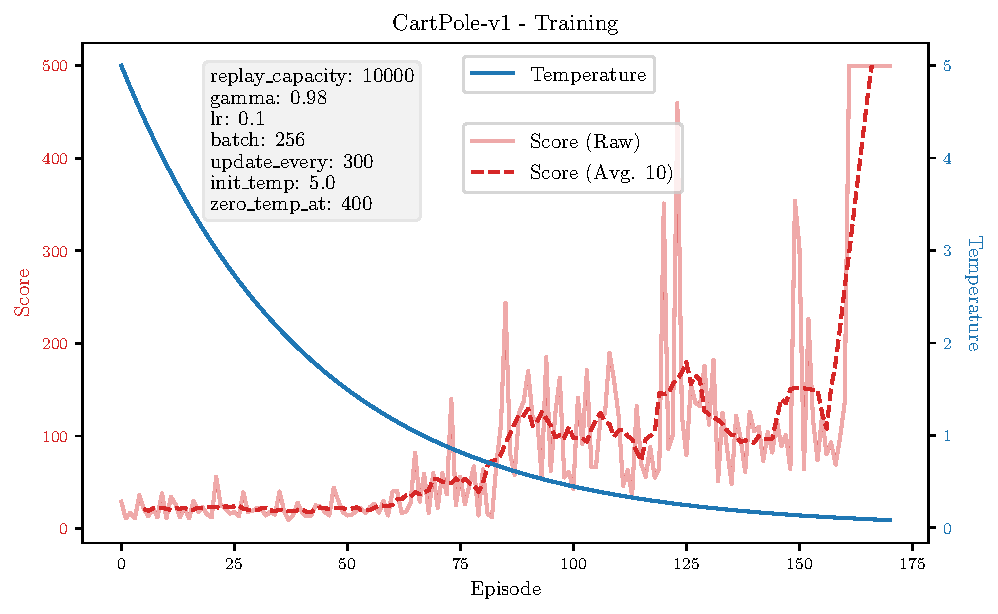
\includegraphics[width=\textwidth]{../Code/Plots/1/24_06_21-00h43m46_best1}
    \caption{Learning curve for CartPole. The temperature is updated at every episode, while the target network is synced every $300$ frames. \label{fig:cartpole_lr}}
\end{figure}

\section{CartPole with Pixels \label{sec:cartpole_pixels}}
The same environment from sec.~\ref{sec:cartpole} is considered. This time, however, the network must learn which features are needed to solve the task directly from an image rendering of the screen. 

\vspace{-.5em}
\subsection{Methods}
The CartPole environment can render the screen as a $600 \times 400$ RGB image. However, most of the pixels are useless to solve the task, since the cart occupies just a small fraction of a frame. Thus, images are preprocessed to reduce their size:
\begin{itemize}
    \item Only the first channel is kept, and it is converted to binary values: $0$ for the background, $1$ for the pixels of the cartpole.
    \item A rectangular region of $200 \times 125$ is cropped around the position of the cart, and eventually padded with zeros to maintain a fixed dimension. In this way, the network will always see the cart as stationary, with only the pole moving. This removes all information about $x_C$ and $\dot{x}_C$. However, a term $-|x_C|$ is still added to the reward (as in sec.~\ref{sec:cartpole}), while $\dot{x}_C$ can be inferred by estimating $\dot{\theta}_P$, and since the cartpole is stationary, the network can easily compute the inclination of the pole. So, effectively, this makes learning easier.
    \item Each sample is a stack of $4$ consecutive frames. In this way, the network has the necessary information to estimate velocities and accelerations.
\end{itemize}

The chosen architecture is taken from the Deepmind paper on Atari games \cite{deepmind_atari}, and consists of two convolutional layers ($16$ filters, kernel $8$ and stride $4$, followed by $32$ filters, kernel $4$ and stride $2$) and a fully-connected layer with $256$ neurons. After each hidden layer a ReLU activation is applied.

A key change from the method of sec.~\ref{sec:cartpole} is the use of Dueling Networks \cite{dueling_networks}. The idea is to follow the convolutional segment with two instances of the fully connected layer. One computes the \textit{advantage} $A(s,a)$ of each action, while the other outputs just a single number, estimating the \textit{value} of the state $V(s)$. The final $Q$-value is then computed as:
\begin{align*}
    Q(s, a) = V(s) + \Big[ A(s,a) - \frac{1}{|\mathcal{A}|} \sum_{a'} A(s,a') \Big]
\end{align*}
where $|\mathcal{A}|$ is the number of actions that the agent $\mathcal{A}$ can perform. Intuitively, this separates the $Q$-value into two terms: the goodness of being in state $s$, and the relative advantage of playing an action $a$. This allows the model to distinguish between \q{hopeless} states where any action will change nothing, and \q{critical} states for which choosing the correct actions matters a lot.

Other than this change, all the considerations from sec.~\ref{sec:cartpole} (e.g. replay memory, exploration profile...) still apply.



\subsection{Results}


The model is trained with the Adam optimizer, and a learning rate of $\lambda = 10^{-4}$, reduced to $\num{0.5e-4}$, $10^{-5}$, $10^{-6}$ or $10^{-7}$ whenever the score surpasses $100$, $200$, $300$ or $400$ respectively.

\begin{figure}[H]
    \centering
    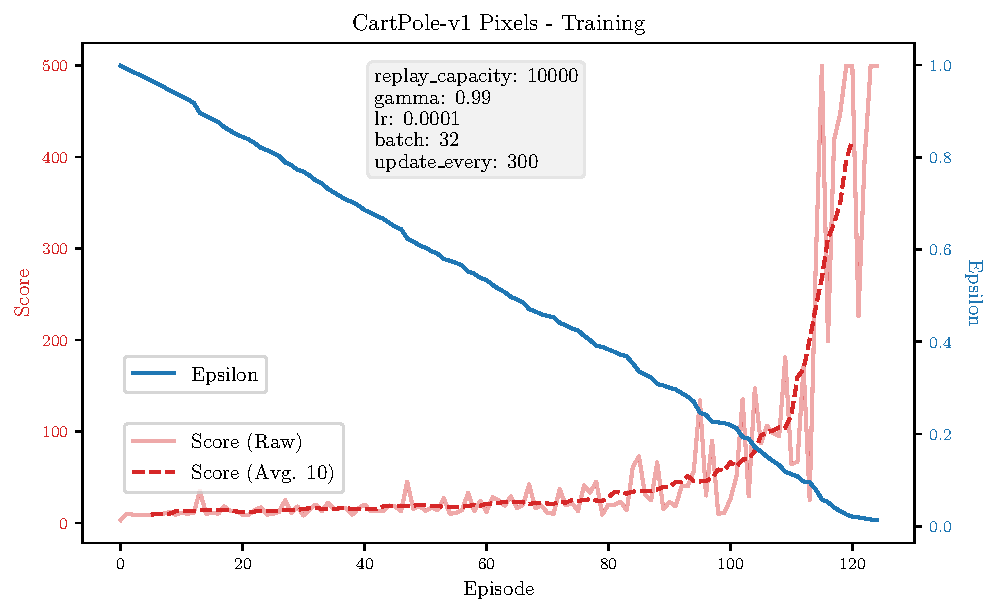
\includegraphics[width=\textwidth]{../Code/Plots/2/25_06_21-02h24m16}
    \caption{Learning curve for CartPole with Pixels. $\epsilon$ is updated at every frame, while the target policy network is updated every $300$ frames. \label{fig:cartpole_pixels_lr}}
\end{figure}

An $\epsilon$-greedy policy is used for exploration, with $\epsilon$ starting from $1$ and decaying exponentially to $0.01$ with a rate of $1/2500$. Differently from sec.~\ref{sec:cartpole}, $\epsilon$ is updated at every frame, and not after each episode. The target network is synced every $300$ frames, and a batch size of $32$ is used. 

\medskip

The learning curve is shown in fig.~\ref{fig:cartpole_pixels_lr}. The model does not completely solve the environment, but still reaches a $475$ mean score over $10$ trials. Video renderings showing its behavior are available at the following \href{https://github.com/Einlar/DLNN_Assignments/tree/main/3/Code/video/02_CartPole_pixels_solved}{link}, along with the network's inputs (files with \texttt{\_cnn}).

\medskip

The main problem seems to be the lack of information about the $x_C$ position, meaning that the cart tends to leave the screen (but maintains the pole upright). However, enforcing the penalty for the cart leaving the center halts the convergence. Similarly, cropping a fixed region that is not centered on the cartpole makes learning extremely difficult. Another issue is that the limited resolution of the rendering means that similar coordinates correspond to the same configuration of pixels, and so the model has access to much less information than that of sec.~\ref{sec:cartpole}.



\section{Pong with Pixels\label{sec:pong}}

\subsection{Methods}
Pong is perhaps the simplest Atari game that can be solved with a DQN. The chosen architecture is the same of sec.~\ref{sec:cartpole_pixels}, which has been proven to work on Atari games in \cite{deepmind_atari}. 

Screen images are used as inputs. They are first converted to grayscale, and then resized to $84\times 84$. One in every $4$ frames is actually shown to the network, with the previous chosen action repeated for the missing frames. This is because Pong games are much longer than CartPole episodes, and do not require frame-perfect moves, meaning that skipping frames is a valid strategy for reducing the computational demand of training. 

Finally, each episode is terminated when the agent loses a single life, as done in \cite{deepmind_nature}. This reduces the amount of frames in each episode, while also priming the agent to avoid losing lives. 

\begin{figure}[H]
    \centering
    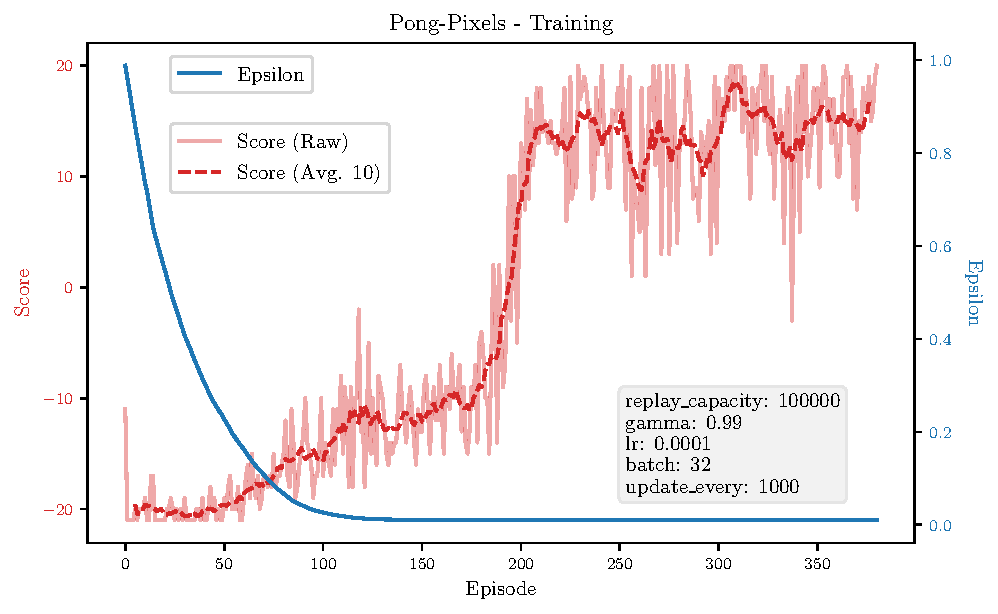
\includegraphics[width=\textwidth]{../Code/Plots/3/25_06_21-22h54m13}
    \caption{Learning curve for Pong with Pixels. $\epsilon$ is updated at every frame, while the target policy network is updated every $1000$ frames. \label{fig:pong_lr}}
\end{figure}

\subsection{Results}
The final model is trained with Adam and a fixed learning rate of $\lambda = 10^{-4}$, a batch size of $32$, and an $\epsilon$-greedy policy for the agent, with $\epsilon$ decreasing exponentially from $1$ to $0.01$ at a rate of $1 / \num{30000}$. As in sec~\ref{sec:cartpole_pixels}, $\epsilon$ is updated at every frame. The target network is synced every $1000$ frames. 

\medskip

The agent starts to beat the baseline opponent after $\sim 200$ episodes. By episode $300$, it achieves superhuman skill, and at the end scores an average of $20$ over $10$ trials (the maximum score in Pong is $21$). In particular, it learns how to reset the game in a specific way, which usually involves losing a life at the very start. Then, it can enter a cycle of moves which guarantees a win against the deterministic opponent. A video rendering of such behavior can be found at the following \href{https://github.com/Einlar/DLNN_Assignments/tree/main/3/Code/video/03_Pong_pixels_solved}{link}.



%\the\textwidth
\printbibliography

\end{document}
